%
% problemstellung.tex 
%
% 
%
% !TEX root = ../../buch.tex
% !TEX encoding = UTF-8
%

\section{Problem\label{antennen:problemstellung}}
\rhead{Problem}
 Es wird versucht eine Antenne zu designen, welche in einem Gerät mit der Form 
 eines Prismas mit Deckfläche eines gleichseitigen Dreiecks. Dies bedeutet, dass 
 die Antenne das Maas eines gleichseitigen Dreiecks nicht überschreiten darf.
 
\subsection{Geometrie\label{antennen:Geom}}
\rhead{Geometrie}
Das Ziel ist nun, den Wirkungsgrad durch Formoptimierung zu erhöhen. 
Die Faktoren k\textsubscript{1} und k\textsubscript{2} sind Konstanten, 
was bedeutet, dass für eine Erhöhung des Wirkungsgrads REF nur die Länge 
l und die Fläche A veränderbar sind. In einem nächsten Schritt wird das Verhältnis
\begin{equation}
	\frac{l}{A^2} \rightarrow \frac{l}{A}
	\label{antennen:Verhältnis}
\end{equation}
% TODO von l/A^2 zu l/A, (beste Fläche auch gleich beste Fläche im Quadrat) + Referenzierung zu Wirkungsgrad
% TODO Diese Formel... danach Besprechung nötig
erhöht. Dieses Verhältnis kann durch die Länge dividiert durch die Fläche 
vereinfacht werden. Diese Formel muss nun auf eine implizite Funktion angewendet 
werden. Eine erste Idee besteht darin, die Ecken abzuflachen, da in den Ecken 
mit viel zusätzlicher Länge nur wenig Fläche gewonnen wird. Zuerst muss eine 
Funktion f(x,y) gefunden werden, welche die Ecken möglichst effizient abflacht. 
Ideen für diese Abflachung sind Geraden wie in Abbildung \ref{antennen:tikabgeflacht} 
zu sehen oder eine Abrundung wie in Abbildung \ref{antennen:tikabgerundet} dargestellt.
 Danach muss bestimmt werden, in welcher Grössenordnung diese Funktion auf das 
 Dreieck " angewendet"  wird. Dies wird in den Abbildungen \ref{antennen:tikabgeflacht_kleiner} 
 und \ref{antennen:tikabgerundet_kleiner} veranschaulicht.

		
\begin{figure}%[htbp]
	\centering
	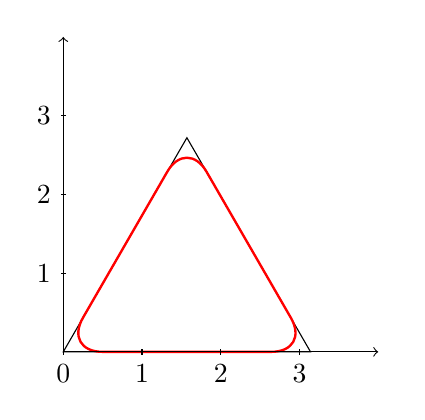
\begin{tikzpicture}
	% Define the length of the sides of the triangles
		\def\sidelength{3.14}
		
	% Calculate the height of the equilateral triangle
		\pgfmathsetmacro{\triangleheight}{sqrt(3)/2*\sidelength}
	% Draw the large outer triangle (white background)
	\draw[fill=white] (0,0) -- (\sidelength,0) -- (0.5*\sidelength, \triangleheight) -- cycle;
		
		% Draw the rounded inner triangle
		\draw[red, line width=0.3mm, rounded corners=0.5cm] (0,0) -- (\sidelength,0) -- (0.5*\sidelength, \triangleheight) -- cycle;
		
		% Draw axes
		\draw[->] (0,0) -- (4,0) node[below right] {};
		\draw[->] (0,0) -- (0,4) node[left] {};
		
		% Add ticks and labels on axes
		\foreach \x in {0, 1,2,3}
		\draw (\x,1pt) -- (\x,-1pt) node[below] {\x};
		\foreach \y in {1, 2, 3}
		\draw (1pt,\y) -- (-1pt,\y) node[left] {\y};
		
	\end{tikzpicture}
	\caption{Antenne mit abgerundeten Ecken}
	\label{antennen:tikabgerundet}
\end{figure}
\begin{figure}%[htbp]
	\centering
	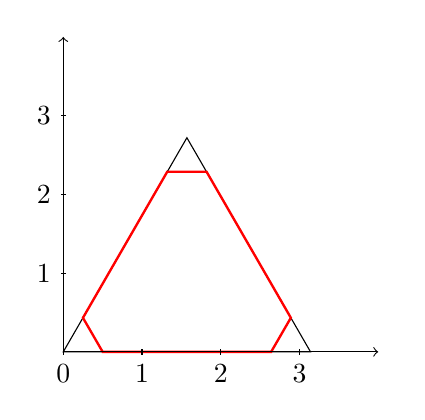
\begin{tikzpicture}
		% Define the length of the sides of the triangles
		\def\sidelength{3.14}
		
		% Calculate the height of the equilateral triangle
		\pgfmathsetmacro{\triangleheight}{sqrt(3)/2*\sidelength}
		% Draw the large outer triangle (white background)
		\draw[fill=white] (0,0) -- (\sidelength,0) -- (0.5*\sidelength, \triangleheight) -- cycle;
		
		% Draw the rounded inner triangle
		\draw[red, line width=0.3mm,] (0.5,0) -- (0.25,1.73 /2*0.5) -- (0.5*\sidelength-0.25, \triangleheight-1.73/2*0.5) -- (0.5*\sidelength+0.25, \triangleheight-1.73/2*0.5)--(\sidelength-0.25,1.73/2*0.5) -- (\sidelength-0.5,0) -- cycle;
		
		% Draw axes
		\draw[->] (0,0) -- (4,0) node[below right] {};
		\draw[->] (0,0) -- (0,4) node[left] {};
		
		% Add ticks and labels on axes
		\foreach \x in {0, 1,2,3}
		\draw (\x,1pt) -- (\x,-1pt) node[below] {\x};
		\foreach \y in {1, 2, 3}
		\draw (1pt,\y) -- (-1pt,\y) node[left] {\y};
		
	\end{tikzpicture}
	\caption{Antenne mit abgeflachten Ecken}
	\label{antennen:tikabgeflacht}
\end{figure}
\begin{figure}%[htbp]
	\centering
	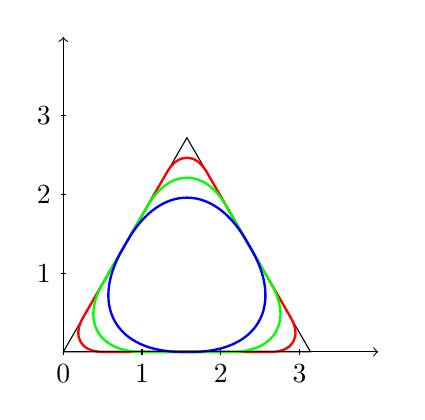
\begin{tikzpicture}
		% Define the length of the sides of the triangles
		\def\sidelength{3.14}
		
		% Calculate the height of the equilateral triangle
		\pgfmathsetmacro{\triangleheight}{sqrt(3)/2*\sidelength}
		% Draw the large outer triangle (white background)
		\draw[fill=white] (0,0) -- (\sidelength,0) -- (0.5*\sidelength, \triangleheight) -- cycle;
		
		% Draw the rounded inner triangle
		\draw[red, line width=0.3mm, rounded corners=0.5cm] (0,0) -- (\sidelength,0) -- (0.5*\sidelength, \triangleheight) -- cycle;
		
		% Draw the rounded inner triangle
		\draw[green, line width=0.3mm, rounded corners=1cm] (0,0) -- (\sidelength,0) -- (0.5*\sidelength, \triangleheight) -- cycle;
		
		% Draw the rounded inner triangle
		\draw[blue, line width=0.3mm, rounded corners=1.5cm] (0,0) -- (\sidelength,0) -- (0.5*\sidelength, \triangleheight) -- cycle;
		
		% Draw axes
		\draw[->] (0,0) -- (4,0) node[below right] {};
		\draw[->] (0,0) -- (0,4) node[left] {};
		
		% Add ticks and labels on axes
		\foreach \x in {0, 1,2,3}
		\draw (\x,1pt) -- (\x,-1pt) node[below] {\x};
		\foreach \y in {1, 2, 3}
		\draw (1pt,\y) -- (-1pt,\y) node[left] {\y};
		
	\end{tikzpicture}
	\caption{Antenne mit abgerundeten Ecken}
	\label{antennen:tikabgerundet_kleiner}
\end{figure}
\begin{figure}%[htbp]
	\centering
	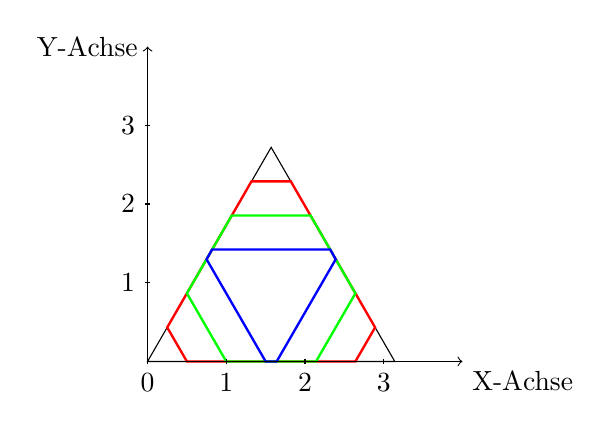
\begin{tikzpicture}
		% Define the length of the sides of the triangles
		\def\sidelength{3.14}
		
		% Calculate the height of the equilateral triangle
		\pgfmathsetmacro{\triangleheight}{sqrt(3)/2*\sidelength}
		% Draw the large outer triangle (white background)
		\draw[fill=white] (0,0) -- (\sidelength,0) -- (0.5*\sidelength, \triangleheight) -- cycle;
		
		% Draw the rounded inner triangle
		\draw[red, line width=0.3mm,] (0.5,0) -- (0.25,1.73 /2*0.5) -- (0.5*\sidelength-0.25, \triangleheight-1.73/2*0.5) -- (0.5*\sidelength+0.25, \triangleheight-1.73/2*0.5)--(\sidelength-0.25,1.73/2*0.5) -- (\sidelength-0.5,0) -- cycle;
		
		% Draw the rounded inner triangle
		\draw[green, line width=0.3mm,] (1,0) -- (0.5,1.73 /2*1) -- (0.5*\sidelength-0.5, \triangleheight-1.73/2*1) -- (0.5*\sidelength+0.5, \triangleheight-1.73/2*1)--(\sidelength-0.5,1.73/2*1) -- (\sidelength-1,0) -- cycle;
		
		% Draw the rounded inner triangle
		\draw[blue, line width=0.3mm,] (1.5,0) -- (0.75,1.73 /2*1.5) -- (0.5*\sidelength-0.75, \triangleheight-1.73/2*1.5) -- (0.5*\sidelength+0.75, \triangleheight-1.73/2*1.5)--(\sidelength-0.75,1.73/2*1.5) -- (\sidelength-1.5,0) -- cycle;
		
		% Draw axes
		\draw[->] (0,0) -- (4,0) node[below right] {X-Achse};
		\draw[->] (0,0) -- (0,4) node[left] {Y-Achse};
		
		% Add ticks and labels on axes
		\foreach \x in {0, 1,2,3}
		\draw (\x,1pt) -- (\x,-1pt) node[below] {\x};
		\foreach \y in {1, 2, 3}
		\draw (1pt,\y) -- (-1pt,\y) node[left] {\y};
		
	\end{tikzpicture}
	\caption{Antenne mit abgeflachten Ecken}
	\label{antennen:tikabgeflacht_kleiner}
\end{figure}
Eine Eigenschaft welche das Problem vereinfacht ist die Symmetrie des Dreiecks. 
Das Gesamtproblem kann vereinfacht werden indem nur eine Ecke betrachtet wird. 
Wie in Abbildung... dargestellt sind die drei Eckfunktionen Äquivalent. Die drei 
gestrichelten Geraden spannen ein weiteres gleichseitiges Dreieck auf, welches 
jedoch vernachlässigt werden kann, da dieses für alle gesuchten Funktionen f(x,y) 
gleich bleibt. Somit ist das implizite Problem f(x,y) zur expliziten Funktion f(x) 
geworden, welche wesentlich leichter zu optimieren ist.











